% Options for packages loaded elsewhere
\PassOptionsToPackage{unicode}{hyperref}
\PassOptionsToPackage{hyphens}{url}
\PassOptionsToPackage{dvipsnames,svgnames,x11names}{xcolor}
%
\documentclass[
  letterpaper,
  DIV=11,
  numbers=noendperiod]{scrartcl}

\usepackage{amsmath,amssymb}
\usepackage{iftex}
\ifPDFTeX
  \usepackage[T1]{fontenc}
  \usepackage[utf8]{inputenc}
  \usepackage{textcomp} % provide euro and other symbols
\else % if luatex or xetex
  \usepackage{unicode-math}
  \defaultfontfeatures{Scale=MatchLowercase}
  \defaultfontfeatures[\rmfamily]{Ligatures=TeX,Scale=1}
\fi
\usepackage{lmodern}
\ifPDFTeX\else  
    % xetex/luatex font selection
\fi
% Use upquote if available, for straight quotes in verbatim environments
\IfFileExists{upquote.sty}{\usepackage{upquote}}{}
\IfFileExists{microtype.sty}{% use microtype if available
  \usepackage[]{microtype}
  \UseMicrotypeSet[protrusion]{basicmath} % disable protrusion for tt fonts
}{}
\makeatletter
\@ifundefined{KOMAClassName}{% if non-KOMA class
  \IfFileExists{parskip.sty}{%
    \usepackage{parskip}
  }{% else
    \setlength{\parindent}{0pt}
    \setlength{\parskip}{6pt plus 2pt minus 1pt}}
}{% if KOMA class
  \KOMAoptions{parskip=half}}
\makeatother
\usepackage{xcolor}
\setlength{\emergencystretch}{3em} % prevent overfull lines
\setcounter{secnumdepth}{5}
% Make \paragraph and \subparagraph free-standing
\ifx\paragraph\undefined\else
  \let\oldparagraph\paragraph
  \renewcommand{\paragraph}[1]{\oldparagraph{#1}\mbox{}}
\fi
\ifx\subparagraph\undefined\else
  \let\oldsubparagraph\subparagraph
  \renewcommand{\subparagraph}[1]{\oldsubparagraph{#1}\mbox{}}
\fi


\providecommand{\tightlist}{%
  \setlength{\itemsep}{0pt}\setlength{\parskip}{0pt}}\usepackage{longtable,booktabs,array}
\usepackage{calc} % for calculating minipage widths
% Correct order of tables after \paragraph or \subparagraph
\usepackage{etoolbox}
\makeatletter
\patchcmd\longtable{\par}{\if@noskipsec\mbox{}\fi\par}{}{}
\makeatother
% Allow footnotes in longtable head/foot
\IfFileExists{footnotehyper.sty}{\usepackage{footnotehyper}}{\usepackage{footnote}}
\makesavenoteenv{longtable}
\usepackage{graphicx}
\makeatletter
\def\maxwidth{\ifdim\Gin@nat@width>\linewidth\linewidth\else\Gin@nat@width\fi}
\def\maxheight{\ifdim\Gin@nat@height>\textheight\textheight\else\Gin@nat@height\fi}
\makeatother
% Scale images if necessary, so that they will not overflow the page
% margins by default, and it is still possible to overwrite the defaults
% using explicit options in \includegraphics[width, height, ...]{}
\setkeys{Gin}{width=\maxwidth,height=\maxheight,keepaspectratio}
% Set default figure placement to htbp
\makeatletter
\def\fps@figure{htbp}
\makeatother

\usepackage{booktabs}
\usepackage{longtable}
\usepackage{array}
\usepackage{multirow}
\usepackage{wrapfig}
\usepackage{float}
\usepackage{colortbl}
\usepackage{pdflscape}
\usepackage{tabu}
\usepackage{threeparttable}
\usepackage{threeparttablex}
\usepackage[normalem]{ulem}
\usepackage{makecell}
\usepackage{xcolor}
\setlength{\tabcolsep}{1pt}
\usepackage{fontspec}
\usepackage{fontawesome}
\setlength{\tabcolsep}{2pt}
\KOMAoption{captions}{tableheading}
\makeatletter
\makeatother
\makeatletter
\makeatother
\makeatletter
\@ifpackageloaded{caption}{}{\usepackage{caption}}
\AtBeginDocument{%
\ifdefined\contentsname
  \renewcommand*\contentsname{Table of contents}
\else
  \newcommand\contentsname{Table of contents}
\fi
\ifdefined\listfigurename
  \renewcommand*\listfigurename{List of Figures}
\else
  \newcommand\listfigurename{List of Figures}
\fi
\ifdefined\listtablename
  \renewcommand*\listtablename{List of Tables}
\else
  \newcommand\listtablename{List of Tables}
\fi
\ifdefined\figurename
  \renewcommand*\figurename{Figure}
\else
  \newcommand\figurename{Figure}
\fi
\ifdefined\tablename
  \renewcommand*\tablename{Table}
\else
  \newcommand\tablename{Table}
\fi
}
\@ifpackageloaded{float}{}{\usepackage{float}}
\floatstyle{ruled}
\@ifundefined{c@chapter}{\newfloat{codelisting}{h}{lop}}{\newfloat{codelisting}{h}{lop}[chapter]}
\floatname{codelisting}{Listing}
\newcommand*\listoflistings{\listof{codelisting}{List of Listings}}
\makeatother
\makeatletter
\@ifpackageloaded{caption}{}{\usepackage{caption}}
\@ifpackageloaded{subcaption}{}{\usepackage{subcaption}}
\makeatother
\makeatletter
\@ifpackageloaded{tcolorbox}{}{\usepackage[skins,breakable]{tcolorbox}}
\makeatother
\makeatletter
\@ifundefined{shadecolor}{\definecolor{shadecolor}{rgb}{.97, .97, .97}}
\makeatother
\makeatletter
\makeatother
\makeatletter
\makeatother
\ifLuaTeX
  \usepackage{selnolig}  % disable illegal ligatures
\fi
\usepackage[authoryear,longnamesfirst]{natbib}
\bibliographystyle{plainnat}
\IfFileExists{bookmark.sty}{\usepackage{bookmark}}{\usepackage{hyperref}}
\IfFileExists{xurl.sty}{\usepackage{xurl}}{} % add URL line breaks if available
\urlstyle{same} % disable monospaced font for URLs
\hypersetup{
  pdftitle={Supplementary materials for: ``Does personal experience of climate change influence climate-change beliefs? The case of the 2019--2020 Australian bushfires''},
  pdfauthor={Matthew Andreotta; Fabio Boschetti; Simon Farrell; Cécile Paris; Iain Walker; Mark Hurlstone},
  colorlinks=true,
  linkcolor={blue},
  filecolor={Maroon},
  citecolor={Blue},
  urlcolor={Blue},
  pdfcreator={LaTeX via pandoc}}

\title{Supplementary materials for: ``Does personal experience of
climate change influence climate-change beliefs? The case of the
2019--2020 Australian bushfires''}
\author{Matthew Andreotta \and Fabio Boschetti \and Simon
Farrell \and Cécile Paris \and Iain Walker \and Mark Hurlstone}
\date{2024-09-27}

\begin{document}
\maketitle
\ifdefined\Shaded\renewenvironment{Shaded}{\begin{tcolorbox}[sharp corners, borderline west={3pt}{0pt}{shadecolor}, interior hidden, boxrule=0pt, enhanced, breakable, frame hidden]}{\end{tcolorbox}}\fi

\hypertarget{methods}{%
\section{Methods}\label{methods}}

\hypertarget{fast-responders}{%
\subsection{Fast responders}\label{fast-responders}}

For each study, a pilot study of approximately fifty people was
conducted to identify fast responders. Fast responders were identified
as those who completed the survey in less than half of the median time
taken by participants in the pilot study, which was 873 seconds for
Study 1, 664 seconds for Study 2, and 509 seconds for Study 3. The data
of fast responders was not collected, and therefore, not included in the
analysis.

\hypertarget{counterbalancing-of-materials}{%
\subsection{Counterbalancing of
materials}\label{counterbalancing-of-materials}}

For Study 1, auxiliary psychological scales were counterbalanced using a
digram-balanced Latin square design. However, there is a slight
discrepancy in the number of each Latin squares completed (range = 25 to
44) due to non-completions and the nature of randomisation. The Q-sort
always preceded the auxiliary psychological scales. Study 3 maintained
this approach to administering materials, to facilitate comparison
between studies. The additional materials (Fire Perception Scale and
Policy direction preferences) were always administered together, and
randomly preceded or proceeded the block of Q-sort and auxiliary
psychological scales. Policy direction preferences always immediately
followed the Fire Perception Scale.

\clearpage

\hypertarget{results}{%
\section{Results}\label{results}}

\hypertarget{segment-membership-replication}{%
\subsection{Segment membership
replication}\label{segment-membership-replication}}

See Table~\ref{tbl-statements}.

\hypertarget{tbl-statements}{}
\begin{longtable}[t]{>{\raggedright\arraybackslash}p{12em}cccccccc}
\caption{\label{tbl-statements}Segment membership factor scores for each study and Q-sort statement }\tabularnewline

\toprule
\multicolumn{1}{c}{ } & \multicolumn{4}{c}{Acceptor} & \multicolumn{4}{c}{Sceptic} \\
\cmidrule(l{3pt}r{3pt}){2-5} \cmidrule(l{3pt}r{3pt}){6-9}
Statement & \parbox{2.5em}{\centering Study 1} & \parbox{2.5em}{\centering Study 2} & \parbox{2.5em}{\centering Study 3} & \parbox{5em}{\centering Maximum difference} & \parbox{2.5em}{\centering Study 1} & \parbox{2.5em}{\centering Study 2} & \parbox{2.5em}{\centering Study 3} & \parbox{5em}{\centering Maximum difference}\\
\midrule
\endfirsthead
\multicolumn{9}{@{}l}{\textit{(continued)}}\\
\toprule
\multicolumn{1}{c}{ } & \multicolumn{4}{c}{Acceptor} & \multicolumn{4}{c}{Sceptic} \\
\cmidrule(l{3pt}r{3pt}){2-5} \cmidrule(l{3pt}r{3pt}){6-9}
Statement & \parbox{2.5em}{\centering Study 1} & \parbox{2.5em}{\centering Study 2} & \parbox{2.5em}{\centering Study 3} & \parbox{5em}{\centering Maximum difference} & \parbox{2.5em}{\centering Study 1} & \parbox{2.5em}{\centering Study 2} & \parbox{2.5em}{\centering Study 3} & \parbox{5em}{\centering Maximum difference}\\
\midrule
\endhead

\endfoot
\bottomrule
\endlastfoot
1. It is important to vote for leaders who will combat climate change. & 4 & 4 & 4 & 0 & -4 & -3 & -4 & 1\\
2. Scientists should stop falsely claiming that climate change is a settled science. & -2 & -2 & -2 & 0 & 4 & 4 & 4 & 0\\
3. Climate change is a hoax perpetrated by the United Nations. & -4 & -4 & -4 & 0 & 3 & 3 & 3 & 0\\
4. Poor people will be impacted the worst by climate change. & 1 & 0 & 1 & 1 & 0 & 0 & 1 & 1\\
5. They changed the name from "global warming" to "climate change" because the planet isn't warming. & -2 & -2 & -2 & 0 & 3 & 3 & 3 & 0\\
6. The concept of global warming was created by and for the Chinese in order to make U.S. manufacturing non-competitive. & -3 & -3 & -3 & 0 & 2 & 1 & 2 & 1\\
7. Cow farts cause more 'climate change' than human activity. & -2 & -2 & -2 & 0 & 1 & 2 & 1 & 1\\
8. Climate change is a threat to the health and safety of our children. & 3 & 3 & 3 & 0 & -3 & -4 & -3 & 1\\
9. Politicians and the mass media are ignorant about the risks of climate change. & 0 & 0 & 0 & 0 & -1 & -1 & -1 & 0\\
10. Climate change sceptics ignore basic climate science facts. & 1 & 1 & 1 & 0 & -1 & -2 & -2 & 1\\
11. Through cutting science funding, we damage Australia's ability to respond to climate change. & 1 & 2 & 2 & 1 & -2 & -1 & -1 & 1\\
12. The Great Barrier Reef is at risk from climate change. & 3 & 3 & 3 & 0 & -2 & -2 & -2 & 0\\
13. The threat of climate change is much worse than climate scientists originally thought. & 2 & 1 & 1 & 1 & -3 & -3 & -3 & 0\\
14. Politicians who refuse to tackle climate change are just as bad as those who deny climate science. & 1 & 1 & 1 & 0 & -1 & -2 & -2 & 1\\
15. The increased occurrence of extreme weather events is a clear sign that climate change is real. & 2 & 2 & 2 & 0 & -2 & -2 & -2 & 0\\
16. Australian agriculture is thriving so climate change can't be real. & -3 & -3 & -3 & 0 & 2 & 2 & 2 & 0\\
17. Australia is experiencing more extreme weather and hotter days due to climate change. & 2 & 2 & 2 & 0 & -2 & -1 & -1 & 1\\
18. Those who demand climate action are the usual "torch-and-pitchfork" crowd. & -2 & -2 & -2 & 0 & 2 & 2 & 2 & 0\\
19. Climate change policy and renewable energy (e.g., solar power) should be a major focus of Australian political elections. & 2 & 2 & 2 & 0 & -1 & 0 & -1 & 1\\
20. Climate sceptics, with no genuine expertise, cannot know better than climate scientists. & 0 & 0 & 0 & 0 & 0 & 0 & 1 & 1\\
21. Climate change and human burning of fossil fuels are strongly linked. & 0 & 1 & 0 & 1 & 0 & -1 & -1 & 1\\
22. People who deny the science of climate change should not hold public office. & 0 & 0 & -1 & 1 & -1 & -1 & 0 & 1\\
23. We need to keep coal, oil, and gas in the ground and adopt more renewable energy sources, like solar and wind power. & 0 & 0 & 0 & 0 & 0 & 0 & 0 & 0\\
24. No political party can say they have a climate change action plan when they favour coal, oil, and gas companies. & -1 & 0 & -1 & 1 & 1 & 1 & 1 & 0\\
25. We must start working together for real solutions on climate change. & 1 & 1 & 1 & 0 & 1 & 1 & 0 & 1\\
26. It is shameful that climate change, the greatest problem of our time, is barely discussed in the media. & -1 & -1 & -1 & 0 & 0 & 0 & 0 & 0\\
27. Countries must fulfil their Paris Climate Agreement goals. & -1 & -1 & 0 & 1 & 1 & 1 & 0 & 1\\
28. Regardless of who is elected, the reality is that climate change is going to destroy everything. & -1 & -1 & -1 & 0 & 0 & 0 & 0 & 0\\
29. Oil and gas companies could not care less about climate change. & -1 & -1 & -1 & 0 & 2 & 2 & 2 & 0\\
30. Australian politicians need to wake up to the emergency of tackling climate change. & 0 & -1 & 0 & 1 & 1 & 1 & 1 & 0\\*
\end{longtable}

\clearpage

\hypertarget{change-in-segment-membership-over-time}{%
\subsection{Change in segment membership over
time}\label{change-in-segment-membership-over-time}}

\hypertarget{multinomial-regression-model}{%
\subsubsection{Multinomial regression
model}\label{multinomial-regression-model}}

We created a multinomial logistic regression model to predict segment
membership as a function of study, using the \emph{multinom} function
from the \emph{nnet} package \citep{venables_2002}. Segment membership
was entered as the dependent variable, with the Fencesitter segment as
the reference category. Study was entered as a categorical predictor,
with Study 2 as the reference category. Coefficients were exponentiated
to estimate odds ratios, and are presented in
Table~\ref{tbl-segment-change}. Coefficient \(p\) values were estimated
using the Wald Z-test.

\hypertarget{tbl-segment-change}{}
\begin{table}
\caption{\label{tbl-segment-change}Estimated effects of study on segment membership using a multinomial
logistic regression model. }\tabularnewline

\centering
\begin{tabular}[t]{>{\raggedright\arraybackslash}p{6em}>{\raggedright\arraybackslash}p{6em}>{\raggedright\arraybackslash}p{6em}>{\raggedright\arraybackslash}p{6em}>{\raggedright\arraybackslash}p{6em}>{\raggedright\arraybackslash}p{6em}}
\toprule
\multicolumn{2}{c}{ } & \multicolumn{2}{c}{\parbox{10em}{\centering Ratio of Acceptor odds and Fencesitter odds}} & \multicolumn{2}{c}{\parbox{10em}{\centering Ratio of Sceptics odds and Fencesitter odds}} \\
\cmidrule(l{3pt}r{3pt}){3-4} \cmidrule(l{3pt}r{3pt}){5-6}
Predictors & Categories & Estimate ($p$ value) & 95\% Confidence interval & Estimate ($p$ value) & 95\% Confidence interval\\
\midrule
Intercept & - & 2.25 (.000)\textsuperscript{***} & {}[1.80, 2.80] & 0.38 (.000)\textsuperscript{***} & {}[0.27, 0.54]\\
Study & Study 1 & 1.06 (.709) & {}[0.78, 1.44] & 0.81 (.417) & {}[0.48, 1.35]\\
 & Study 2 & - & - & - & -\\
 & Study 3 & 0.65 (.021)\textsuperscript{*} & {}[0.46, 0.94] & 0.60 (.111) & {}[0.32, 1.12]\\
\bottomrule
\multicolumn{6}{l}{\rule{0pt}{1em}\textit{Note: }}\\
\multicolumn{6}{l}{\rule{0pt}{1em}\textsuperscript{*}\textit{p} $<$ .05; \textsuperscript{***}\textit{p} $<$ .001.}\\
\multicolumn{6}{l}{\rule{0pt}{1em}\parbox{36em}{Each study was entered as a categorical predictor, with Study 2 as the reference category. Model estimates of coefficients were exponentiated to odds ratios.}}\\
\end{tabular}
\end{table}

\clearpage

\hypertarget{auxiliary-psychological-characteristics}{%
\subsection{Auxiliary psychological
characteristics}\label{auxiliary-psychological-characteristics}}

See Table~\ref{tbl-mean_diff} for the difference in means of auxiliary
psychological characteristics between Study 1 and Study 3, for:
cognitive style; ideology, worldviews, and values; and personality.

See Figure~\ref{fig-scale-change} for density estimates of auxiliary
psychological characteristics in Study 1 and Study 3.

\hypertarget{tbl-mean_diff}{}
\begin{table}
\caption{\label{tbl-mean_diff}Difference in means of auxiliary psychological characteristics over
time. }\tabularnewline

\centering
\begin{tabular}[t]{l>{\raggedright\arraybackslash}p{5em}>{\raggedright\arraybackslash}p{5em}>{\raggedright\arraybackslash}p{2.5em}>{\raggedright\arraybackslash}p{3em}>{\raggedright\arraybackslash}p{4em}}
\toprule
\multicolumn{1}{c}{ } & \multicolumn{1}{c}{\parbox{4em}{Study 1}} & \multicolumn{1}{c}{\parbox{4em}{Study 3}} & \multicolumn{3}{c}{ } \\
\cmidrule(l{3pt}r{3pt}){2-2} \cmidrule(l{3pt}r{3pt}){3-3}
Psychological characteristics & \textit{M} (\textit{SD}) & \textit{M} (\textit{SD}) & \textit{t} & \textit{p} & $p_{adjusted}$\\
\midrule
\addlinespace[0.3em]
\multicolumn{6}{l}{\textbf{Cognitive style}}\\
\hspace{1em}Orientation to Immediate Goals & 2.57 (0.91) & 2.74 (0.87) & 2.36 & .019 & .08\\
\hspace{1em}Conspiracist Ideation & 2.32 (1.02) & 2.45 (1.11) & 1.41 & .158 & .47\\
\hspace{1em}Need for Cognition & 3.36 (0.78) & 3.37 (0.76) & 0.12 & .901 & 1.00\\
\hspace{1em}Orientation to Future Goals & 3.74 (0.68) & 3.74 (0.73) & -0.07 & .943 & 1.00\\
\addlinespace[0.3em]
\multicolumn{6}{l}{\textbf{Ideology, worldviews, and values}}\\
\hspace{1em}Environment-as-Elastic Worldview & 2.44 (0.92) & 2.62 (0.92) & 2.37 & .018 & .11\\
\hspace{1em}Political Ideology & 3.62 (1.59) & 3.89 (1.39) & 2.21 & .028 & .14\\
\hspace{1em}System Justification & 5.00 (1.58) & 5.20 (1.44) & 1.59 & .113 & .45\\
\hspace{1em}Self-Transcendence Values & -0.34 (0.97) & -0.44 (0.95) & -1.27 & .204 & .61\\
\hspace{1em}Conservation Values & 1.31 (0.91) & 1.36 (0.91) & 0.61 & .539 & 1.00\\
\hspace{1em}Environment-as-Ductile Worldview & 3.76 (0.75) & 3.76 (0.71) & -0.01 & .994 & 1.00\\
\addlinespace[0.3em]
\multicolumn{6}{l}{\textbf{Personality}}\\
\hspace{1em}Conscientiousness & 3.76 (0.89) & 3.71 (0.84) & -0.72 & .469 & 1.00\\
\hspace{1em}Agreeableness & 3.62 (0.84) & 3.58 (0.87) & -0.57 & .571 & 1.00\\
\hspace{1em}Extraversion & 2.85 (0.96) & 2.83 (0.97) & -0.28 & .776 & 1.00\\
\hspace{1em}Openness & 3.32 (0.84) & 3.33 (0.80) & 0.13 & .893 & 1.00\\
\hspace{1em}Neuroticism & 2.77 (1.06) & 2.77 (1.00) & -0.02 & .987 & 1.00\\
\bottomrule
\multicolumn{6}{l}{\rule{0pt}{1em}\textit{Note: }}\\
\multicolumn{6}{l}{\rule{0pt}{1em}\parbox{36em}{\textit{p} values were adjusted using the \citet{holm1979} method.}}\\
\end{tabular}
\end{table}

\begin{figure}

{\centering 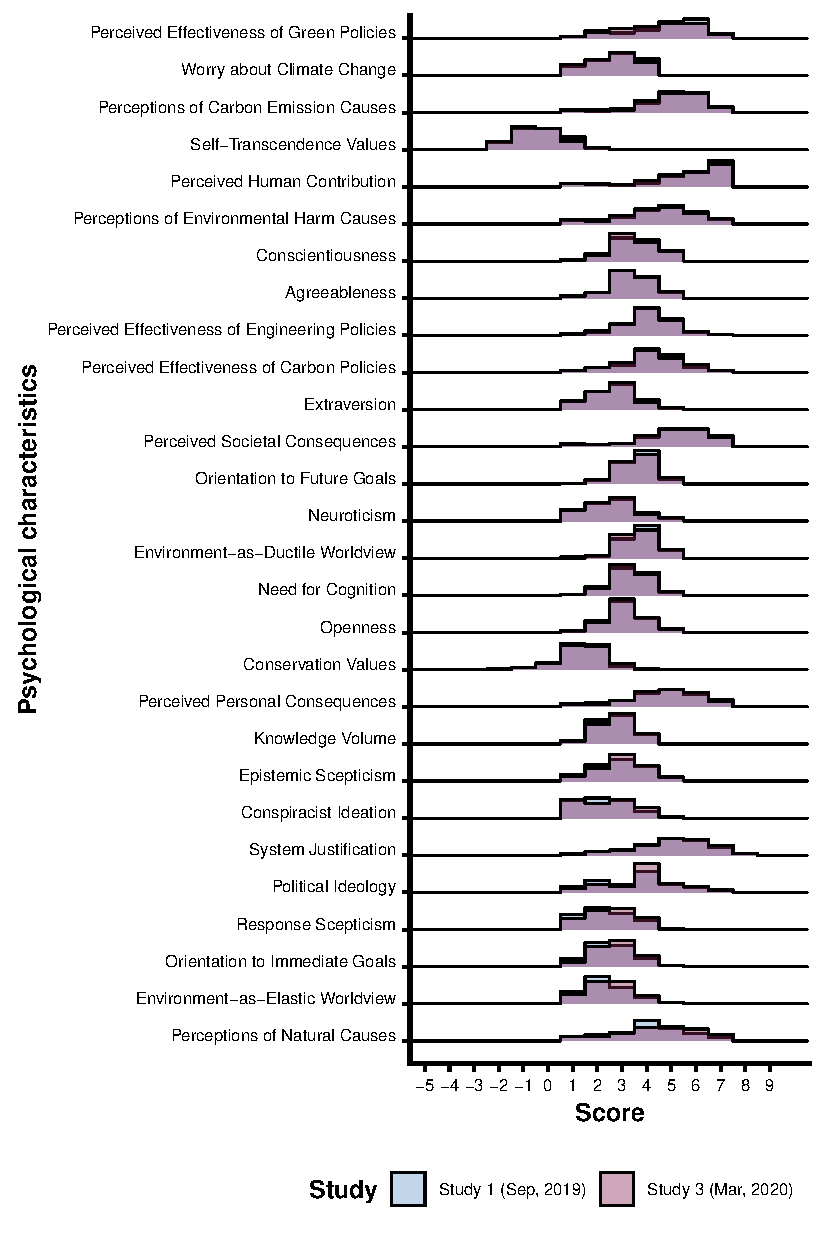
\includegraphics{supplement_files/figure-pdf/fig-scale-change-1.pdf}

}

\caption{\label{fig-scale-change}Density estimates for auxiliary
psychological variables in Study 1 (blue) and Study 3 (purple).}

\end{figure}

\clearpage

\hypertarget{fire-perception-scale}{%
\subsection{Fire Perception Scale}\label{fire-perception-scale}}

\hypertarget{scree-plot}{%
\subsubsection{Scree plot}\label{scree-plot}}

The scree plot for the Fire Perception Scale is shown in
Figure~\ref{fig-fps-scree}.

\begin{figure}

{\centering 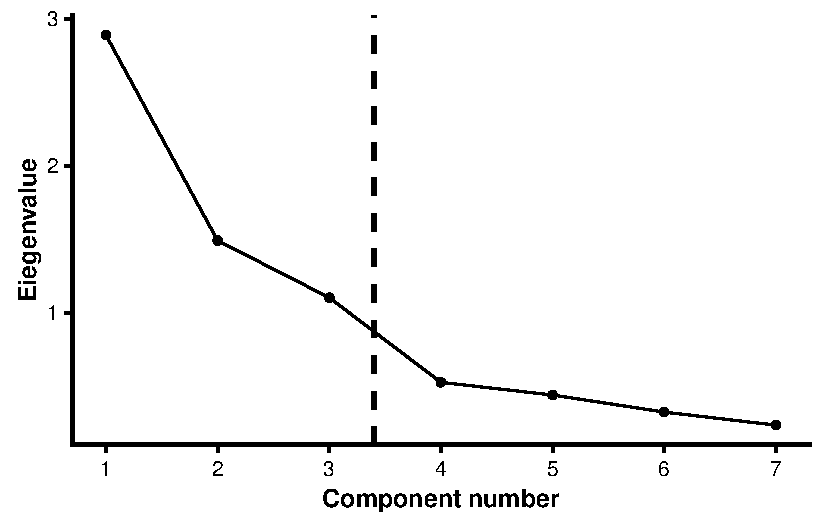
\includegraphics{supplement_files/figure-pdf/fig-fps-scree-1.pdf}

}

\caption{\label{fig-fps-scree}Scree plot for the Fire Perception Scale.
Vertical dashed line indicates a break in the scree.}

\end{figure}

\hypertarget{segment-differences}{%
\subsubsection{Segment differences}\label{segment-differences}}

For each Fire Perception Scale subscale (climate processes, fire
realities, and arson causes), we built a linear regression model to
predict subscale score as a function of segment, using the \emph{lm}
function from the \emph{stats} package \citep{rcoreteam_2023}. Segment
was entered as a categorical predictor, and a Wald Z-test was used to
estimate \(p\) values (Table~\ref{tbl-fps-models}).

\hypertarget{tbl-fps-models}{}
\begin{table}
\caption{\label{tbl-fps-models}Linear regression models predicting Fire Perception Scale subscale
scores (bolded) as a function of segment. }\tabularnewline

\centering
\begin{tabular}[t]{>{\raggedright\arraybackslash}p{13em}l>{\raggedright\arraybackslash}p{7em}>{\raggedright\arraybackslash}p{6em}}
\toprule
Models and predictors & Categories & Estimate ($p$ value) & 95\% Confidence interval\\
\midrule
\addlinespace[0.3em]
\multicolumn{4}{l}{\textbf{(A) Climate Processes}}\\
\hspace{1em}Intercept & - & 2.95 (.000)\textsuperscript{***} & {}[2.74, 3.16]\\
\hspace{1em}Segment & Acceptors & 0.53 (.000)\textsuperscript{***} & {}[0.26, 0.80]\\
\hspace{1em} & Fencesitters & - & \vphantom{2} -\\
\hspace{1em} & Sceptics & -1.76 (.000)\textsuperscript{***} & {}[-2.24, -1.27]\\
\addlinespace[0.3em]
\multicolumn{4}{l}{\textbf{(B) Fire Realities}}\\
\hspace{1em}Intercept & - & 3.66 (.000)\textsuperscript{***} & {}[3.50, 3.83]\\
\hspace{1em}Segment & Acceptors & 0.84 (.000)\textsuperscript{***} & {}[0.63, 1.06]\\
\hspace{1em} & Fencesitters & - & \vphantom{1} -\\
\hspace{1em} & Sceptics & 0.36 (.064) & {}[-0.02, 0.75]\\
\addlinespace[0.3em]
\multicolumn{4}{l}{\textbf{(C) Arson Causes}}\\
\hspace{1em}Intercept & - & 3.71 (.000)\textsuperscript{***} & {}[3.46, 3.96]\\
\hspace{1em}Segment & Acceptors & -0.55 (.001)\textsuperscript{**} & {}[-0.88, -0.23]\\
\hspace{1em} & Fencesitters & - & -\\
\hspace{1em} & Sceptics & 0.74 (.014)\textsuperscript{*} & {}[0.15, 1.32]\\
\bottomrule
\multicolumn{4}{l}{\rule{0pt}{1em}\textit{Note: }}\\
\multicolumn{4}{l}{\rule{0pt}{1em}\textsuperscript{*}\textit{p} $<$ .05; \textsuperscript{**}\textit{p} $<$ .01; \textsuperscript{***}\textit{p} $<$ .001.}\\
\multicolumn{4}{l}{\rule{0pt}{1em}\parbox{30em}{Each segment was entered as a categorical predictor, with Fencesitter as the reference category.}}\\
\end{tabular}
\end{table}

\hypertarget{correlations}{%
\subsubsection{Correlations}\label{correlations}}

The correlations between the Fire Perception Scale subscale scores and
auxiliary psychological characteristics are shown in
Table~\ref{tbl-fps-correlations}.

\hypertarget{tbl-fps-correlations}{}
\begin{table}
\caption{\label{tbl-fps-correlations}Pearson correlations between the Fire Perception Scale subscale scores
and auxiliary psychological characteristics. }\tabularnewline

\centering
\begin{tabular}[t]{l>{\raggedright\arraybackslash}p{6em}>{\raggedright\arraybackslash}p{6em}>{\raggedright\arraybackslash}p{6em}}
\toprule
\multicolumn{1}{c}{ } & \multicolumn{3}{c}{Fire Perception Scale} \\
\cmidrule(l{3pt}r{3pt}){2-4}
Psychological characteristics & (A) Climate Processes & (B) Fire Realities & (C) Arson Causes\\
\midrule
\addlinespace[0.3em]
\multicolumn{4}{l}{\textbf{Climate change cognition and affect}}\\
\hspace{1em}Epistemic Scepticism & \textcolor[HTML]{BAC183}{-0.48\textsuperscript{***}} & \textcolor[HTML]{D1D4A4}{-0.31\textsuperscript{***}} & \textcolor[HTML]{ECB9BB}{0.41\textsuperscript{***}}\\
\hspace{1em}Response Scepticism & \textcolor[HTML]{C4C991}{-0.41\textsuperscript{***}} & \textcolor[HTML]{C2C78F}{-0.43\textsuperscript{***}} & \textcolor[HTML]{F1CBC6}{0.30\textsuperscript{***}}\\
\hspace{1em}Perceptions of Natural Causes & \textcolor[HTML]{FAEFDD}{0.07} & \textcolor[HTML]{D7D9AC}{-0.28\textsuperscript{***}} & \textcolor[HTML]{F3D3CB}{0.25\textsuperscript{***}}\\
\hspace{1em}Perceived Societal Consequences & \textcolor[HTML]{D46780}{0.62\textsuperscript{***}} & \textcolor[HTML]{F6E1D4}{0.16\textsuperscript{*}} & \textcolor[HTML]{DFE0B8}{-0.22\textsuperscript{**}}\\
\hspace{1em}Perceived Human Contribution & \textcolor[HTML]{D46780}{0.64\textsuperscript{***}} & \textcolor[HTML]{F4D9CF}{0.22\textsuperscript{**}} & \textcolor[HTML]{E3E4BE}{-0.18\textsuperscript{**}}\\
\hspace{1em}Perceived Effectiveness of Engineering Policies & \textcolor[HTML]{E0E1BA}{-0.21\textsuperscript{**}} & \textcolor[HTML]{F1CCC7}{0.30\textsuperscript{***}} & \textcolor[HTML]{EEEDCE}{-0.11}\\
\hspace{1em}Perceived Personal Consequences & \textcolor[HTML]{D46780}{0.64\textsuperscript{***}} & \textcolor[HTML]{FDFBE4}{0.01} & \textcolor[HTML]{E7E7C4}{-0.16\textsuperscript{*}}\\
\hspace{1em}Perceptions of Carbon Emission Causes & \textcolor[HTML]{D46780}{0.66\textsuperscript{***}} & \textcolor[HTML]{FBF4E0}{0.04} & \textcolor[HTML]{E8E9C6}{-0.15\textsuperscript{*}}\\
\hspace{1em}Perceived Effectiveness of Green Policies & \textcolor[HTML]{F3F2D6}{-0.07} & \textcolor[HTML]{EFC4C2}{0.35\textsuperscript{***}} & \textcolor[HTML]{EBEBCA}{-0.13}\\
\hspace{1em}Perceived Effectiveness of Carbon Policies & \textcolor[HTML]{EBEBCA}{-0.12} & \textcolor[HTML]{F0C6C3}{0.33\textsuperscript{***}} & \textcolor[HTML]{EFEFD0}{-0.09}\\
\hspace{1em}Worry about Climate Change & \textcolor[HTML]{D46780}{0.64\textsuperscript{***}} & \textcolor[HTML]{FBF9E2}{0.00} & \textcolor[HTML]{EEEDCE}{-0.11}\\
\hspace{1em}Knowledge Volume & \textcolor[HTML]{F7E4D6}{0.14\textsuperscript{*}} & \textcolor[HTML]{F9EBDA}{0.10} & \textcolor[HTML]{FAEFDD}{0.07}\\
\hspace{1em}Perceptions of Environmental Harm Causes & \textcolor[HTML]{E5A5AF}{0.54\textsuperscript{***}} & \textcolor[HTML]{EFEFD0}{-0.10} & \textcolor[HTML]{F2F1D4}{-0.07}\\
\addlinespace[0.3em]
\multicolumn{4}{l}{\textbf{Cognitive style}}\\
\hspace{1em}Conspiracist Ideation & \textcolor[HTML]{FAF1DE}{0.07} & \textcolor[HTML]{D7D9AC}{-0.28\textsuperscript{***}} & \textcolor[HTML]{F2D1CA}{0.26\textsuperscript{***}}\\
\hspace{1em}Orientation to Future Goals & \textcolor[HTML]{EFC4C2}{0.35\textsuperscript{***}} & \textcolor[HTML]{F7E3D5}{0.16\textsuperscript{*}} & \textcolor[HTML]{F4F3D8}{-0.05}\\
\hspace{1em}Orientation to Immediate Goals & \textcolor[HTML]{FBF6E1}{0.04} & \textcolor[HTML]{CBCE9A}{-0.36\textsuperscript{***}} & \textcolor[HTML]{F7E3D5}{0.15\textsuperscript{*}}\\
\hspace{1em}Need for Cognition & \textcolor[HTML]{F9ECDB}{0.10} & \textcolor[HTML]{F7E3D5}{0.16\textsuperscript{*}} & \textcolor[HTML]{F6F4DA}{-0.04}\\
\addlinespace[0.3em]
\multicolumn{4}{l}{\textbf{Ideology, worldviews, or values}}\\
\hspace{1em}Environment-as-Elastic Worldview & \textcolor[HTML]{D1D4A4}{-0.32\textsuperscript{***}} & \textcolor[HTML]{C0C58B}{-0.45\textsuperscript{***}} & \textcolor[HTML]{F4D8CE}{0.22\textsuperscript{**}}\\
\hspace{1em}Self-Transcendence Values & \textcolor[HTML]{D3D5A6}{-0.30\textsuperscript{***}} & \textcolor[HTML]{F2CEC8}{0.29\textsuperscript{***}} & \textcolor[HTML]{F3F2D6}{-0.06}\\
\hspace{1em}Conservation Values & \textcolor[HTML]{DFE0B8}{-0.22\textsuperscript{**}} & \textcolor[HTML]{D5D8AA}{-0.28\textsuperscript{***}} & \textcolor[HTML]{F2D1CA}{0.27\textsuperscript{***}}\\
\hspace{1em}Environment-as-Ductile Worldview & \textcolor[HTML]{E8AEB4}{0.49\textsuperscript{***}} & \textcolor[HTML]{F3D4CC}{0.24\textsuperscript{***}} & \textcolor[HTML]{EBEBCA}{-0.13}\\
\hspace{1em}Political Ideology & \textcolor[HTML]{DCDEB4}{-0.24\textsuperscript{***}} & \textcolor[HTML]{DCDEB4}{-0.23\textsuperscript{***}} & \textcolor[HTML]{F2D0C9}{0.28\textsuperscript{***}}\\
\hspace{1em}System Justification & \textcolor[HTML]{FBF3DF}{0.05} & \textcolor[HTML]{E6E6C2}{-0.16\textsuperscript{*}} & \textcolor[HTML]{F3D4CC}{0.24\textsuperscript{***}}\\
\addlinespace[0.3em]
\multicolumn{4}{l}{\textbf{Personality}}\\
\hspace{1em}Conscientiousness & \textcolor[HTML]{ECECCC}{-0.11} & \textcolor[HTML]{F9EBDA}{0.10} & \textcolor[HTML]{FBF6E1}{0.04}\\
\hspace{1em}Neuroticism & \textcolor[HTML]{F8E7D8}{0.12} & \textcolor[HTML]{EFEFD0}{-0.10} & \textcolor[HTML]{FBF3DF}{0.05}\\
\hspace{1em}Openness & \textcolor[HTML]{FCF9E3}{0.01} & \textcolor[HTML]{F9EBDA}{0.10} & \textcolor[HTML]{F3F2D6}{-0.06}\\
\hspace{1em}Extraversion & \textcolor[HTML]{F8F7DE}{-0.02} & \textcolor[HTML]{F3F2D6}{-0.06} & \textcolor[HTML]{FCF7E2}{0.03}\\
\hspace{1em}Agreeableness & \textcolor[HTML]{FAF8E0}{-0.01} & \textcolor[HTML]{F9ECDB}{0.10} & \textcolor[HTML]{F8F7DE}{-0.02}\\
\bottomrule
\multicolumn{4}{l}{\rule{0pt}{1em}\textit{Note: }}\\
\multicolumn{4}{l}{\rule{0pt}{1em}\textsuperscript{*}\textit{p} $<$ .05; \textsuperscript{**}\textit{p} $<$ .01; \textsuperscript{***}\textit{p} $<$ .001.}\\
\multicolumn{4}{l}{\rule{0pt}{1em}\parbox{30em}{Colour indicates the magnitude and direction of the correlation.}}\\
\end{tabular}
\end{table}

\clearpage

\hypertarget{policy-direction-preferences}{%
\subsection{Policy direction
preferences}\label{policy-direction-preferences}}

\hypertarget{policy-direction-preferences-as-a-function-of-segment-membership}{%
\subsubsection{Policy direction preferences as a function of segment
membership}\label{policy-direction-preferences-as-a-function-of-segment-membership}}

To assess the association between segment membership and policy
direction preferences, we used a binomial logistic regression model (see
Table~\ref{tbl-policy-preferences}). Policy direction preferences were
coded as a binary variable, with 1 indicating a preference for more
action and 0 indicating an alternative preference (e.g., a preference
for no change, less action, or no action). The model estimated the log
odds ratio of a preference for more action as a function of segment
membership, using the \emph{glm} function with a logit link function.
Association between segment membership and the use of emotional words
was assessed with a likelihood-ratio test that compared the regression
model with and without segment membership as a predictor (\(\chi^{2}\)
(1) = 35.45, \(p\) \textless{} .001). A Wald Z-test was used to estimate
\(p\) values of model coefficients. As no Sceptic indicated a preference
for more action, we could not estimate the effect of segment membership
on policy direction preferences for Sceptic and therefore excluded
Sceptic from the model.

\hypertarget{tbl-policy-preferences}{}
\begin{table}
\caption{\label{tbl-policy-preferences}Estimated effects of segment membership on policy direction preferences
using a binomial logistic regression model. }\tabularnewline

\centering
\begin{tabular}[t]{>{\raggedright\arraybackslash}p{7em}>{\raggedright\arraybackslash}p{7em}>{\raggedright\arraybackslash}p{10em}>{\raggedright\arraybackslash}p{10em}}
\toprule
\multicolumn{2}{c}{ } & \multicolumn{2}{c}{\parbox{19em}{\centering Ratio of the odds of a preference for more action and the odds of an alternative preference}} \\
\cmidrule(l{3pt}r{3pt}){3-4}
Predictors & Categories & Estimate ($p$ value) & 95\% Confidence interval\\
\midrule
Intercept & - & 1.08 (.736) & {}[0.69, 1.68]\\
Segment & Acceptors & 8.03 (.000)\textsuperscript{***} & {}[3.92, 17.49]\\
 & Fencesitters & - & -\\
\bottomrule
\multicolumn{4}{l}{\rule{0pt}{1em}\textit{Note: }}\\
\multicolumn{4}{l}{\rule{0pt}{1em}\textsuperscript{***}\textit{p} $<$ .001.}\\
\multicolumn{4}{l}{\rule{0pt}{1em}\parbox{34em}{Each segment was entered as a categorical predictor, with Fencesitter as the reference category. Sceptics were excluded from the model, as none indicated a preference for more action. Model estimates of coefficients were exponentiated to odds ratios.}}\\
\end{tabular}
\end{table}

\hypertarget{emotion-analysis}{%
\subsubsection{Emotion analysis}\label{emotion-analysis}}

To explore the relationship between segment membership and policy
direction preferences, we conducted an emotion analysis of participants'
justifications for their policy direction preferences. First, we
prepared the data by segmenting each participant's text response into
individual words (known as tokenisation), via the \emph{unnest\_tokens}
function of the \emph{tidytext} package \citep{silge_2016}. Then, we
removed words that were not relevant to the analysis, such as numbers,
hyperlinks, and hashtags. Additionally, we removed words with a unique
meaning in the context of the study, including ``climate'', ``change'',
``global'', ``warming'', ``bushfire'', ``bushfires'', ``fires'',
``fire'', ``barrier'' and ``bark''. Next, we identified the words
present in the NRC Word-Emotion Association Lexicon
\citep{mohammad_2013}. Due to the infrequent use of emotional language
by participants, we examine whether a participant used one or more words
associated with a particular emotion. The resulting prevalence of
emotions in participants' justifications is shown in
Table~\ref{tbl-sentiment-counts}.

To explore segment differences in the use of emotional language, we
created a binomial logistic regression model
(Table~\ref{tbl-sentiment-models}). The model estimated the log odds
ratio of using an emotion, using the \emph{glm} function with a logit
link function. Segment membership was entered as a categorical
predictor, with Fencesitter as the reference category. Association
between segment membership and the use of emotional words was assessed
with a likelihood-ratio test that compared the regression model with and
without segment membership as a predictor. To control for multiple
comparisons, the \(p\) values of likelihood-ratio tests were adjusted
using the Holm \citeyearpar{holm1979} method. A Wald Z-test was used to
estimate the (unadjusted) \(p\) values of model coefficients. We
followed up significant results with pairwise comparisons between
segments, using the \emph{marginaleffects} package
\citep{R-marginaleffects} Table~\ref{tbl-sentiment-models-contrasts}
with a Holm \citeyearpar{holm1979} \(p\) value adjustment for multiple
comparisons.

\hypertarget{tbl-sentiment-counts}{}
\begin{table}
\caption{\label{tbl-sentiment-counts}Frequency and proportion of participants' emotions in justification of
policy direction preferences. }\tabularnewline

\centering
\begin{tabular}[t]{lcc>{\raggedright\arraybackslash}p{23em}}
\toprule
Emotion & \textit{n} & \parbox{7em}{\centering Proportion of sample (\%)} & Example response\\
\midrule
Fear & 67 & 31.46 & ``the recent bushfire is a wakeup call. how much more \textbf{worse} do we want to experience?''\\
Trust & 54 & 25.35 & ``they keep stating that they in front Paris \textbf{agreement,} but this \textbf{agreement} isn't enough, the way the world is going these environment issue will get worse''\\
Anticipation & 42 & 19.72 & ``It is \textbf{expected} of them, and facing re election they need to show they are doing something''\\
Sadness & 41 & 19.25 & ``because forest fires has causing \textbf{negative} consequences''\\
Anger & 31 & 14.55 & ``We are \textbf{destroying} our home and recent weather patterns confirm we are going to \textbf{lose} our home''\\
Disgust & 23 & 10.80 & ``i dont think the climate change has much to do with the fires thats all up to the \textbf{nasty} people thats started them''\\
Surprise & 21 & 9.86 & ``No such thing as climate change. Ever since God created the Earth it has heated and cooled. And Jesus shall return soon.What is coming those who do not believe are in for a \textbf{shock}''\\
Joy & 17 & 7.98 & ``few steps are taken, but there is a big \textbf{journey} ahead of us''\\
\bottomrule
\multicolumn{4}{l}{\rule{0pt}{1em}\textit{Note: }}\\
\multicolumn{4}{l}{\rule{0pt}{1em}Bolded words reflect the exemplified emotion.}\\
\end{tabular}
\end{table}

\hypertarget{tbl-sentiment-models}{}
\begin{longtable}[t]{>{\raggedright\arraybackslash}p{7em}>{\raggedright\arraybackslash}p{7em}>{\raggedright\arraybackslash}p{10em}>{\raggedright\arraybackslash}p{10em}}
\caption{\label{tbl-sentiment-models}Effects of segment membership on emotion content in justification of
policy direction preferences, estimated using a binomial logistic
regression model. }\tabularnewline

\toprule
\multicolumn{2}{c}{ } & \multicolumn{2}{c}{\parbox{19em}{\centering Ratio of the odds of an emotion word present and the odds of an emotion word absent}} \\
\cmidrule(l{3pt}r{3pt}){3-4}
Predictors & Categories & Estimate ($p$ value) & 95\% Confidence interval\\
\midrule
\endfirsthead
\multicolumn{4}{@{}l}{\textit{(continued)}}\\
\toprule
\multicolumn{2}{c}{ } & \multicolumn{2}{c}{\parbox{19em}{\centering Ratio of the odds of an emotion word present and the odds of an emotion word absent}} \\
\cmidrule(l{3pt}r{3pt}){3-4}
Predictors & Categories & Estimate ($p$ value) & 95\% Confidence interval\\
\midrule
\endhead

\endfoot
\bottomrule
\multicolumn{4}{l}{\rule{0pt}{1em}\textit{Note: }}\\
\multicolumn{4}{l}{\rule{0pt}{1em}\textsuperscript{*}\textit{p} $<$ .05; \textsuperscript{**}\textit{p} $<$ .01; \textsuperscript{***}\textit{p} $<$ .001.}\\
\multicolumn{4}{l}{\rule{0pt}{1em}\parbox{32em}{Each segment was entered as a categorical predictor, with Fencesitter as the reference category. The $\chi^{2}$ statistic is the likelihood-ratio test comparing the model with segment as a predictor to the null model without the predictor. The likelihood-ratio test \textit{p} values were adjusted using the \citet{holm1979} method. Model estimates of coefficients were exponentiated to odds ratios.}}\\
\endlastfoot
\addlinespace[0.3em]
\multicolumn{4}{l}{\textbf{Anger ($\chi^{2}$ (2) = 8.73, $p$ = .013, $p_{adjusted}$ = .056)}}\\
\hspace{1em}Intercept & - & 0.10 (.000)\textsuperscript{***} & {}[0.04, 0.20]\\
\hspace{1em}Segment & Acceptors & 1.77 (.231) & {}[0.72, 4.77]\\
\hspace{1em}Segment & Fencesitters & - & \vphantom{5} -\\
\hspace{1em}Segment & Sceptics & 6.55 (.003)\textsuperscript{**} & {}[1.91, 22.94]\\
\addlinespace[0.3em]
\multicolumn{4}{l}{\textbf{Fear ($\chi^{2}$ (2) = 11.93, $p$ = .003, $p_{adjusted}$ = .015*)}}\\
\hspace{1em}Intercept & - & 0.22 (.000)\textsuperscript{***} & {}[0.12, 0.37]\\
\hspace{1em}Segment & Acceptors & 3.16 (.001)\textsuperscript{**} & {}[1.63, 6.46]\\
\hspace{1em}Segment & Fencesitters & - & \vphantom{4} -\\
\hspace{1em}Segment & Sceptics & 2.32 (.147) & {}[0.71, 7.13]\\
\addlinespace[0.3em]
\multicolumn{4}{l}{\textbf{Anticipation ($\chi^{2}$ (2) = 1.18, $p$ = .554, $p_{adjusted}$ = 1.000)}}\\
\hspace{1em}Intercept & - & 0.20 (.000)\textsuperscript{***} & {}[0.10, 0.34]\\
\hspace{1em}Segment & Acceptors & 1.47 (.309) & {}[0.71, 3.14]\\
\hspace{1em}Segment & Fencesitters & - & \vphantom{3} -\\
\hspace{1em}Segment & Sceptics & 1.02 (.983) & {}[0.21, 3.65]\\
\addlinespace[0.3em]
\multicolumn{4}{l}{\textbf{Joy ($\chi^{2}$ (2) = 1.65, $p$ = .437, $p_{adjusted}$ = 1.000)}}\\
\hspace{1em}Intercept & - & 0.08 (.000)\textsuperscript{***} & {}[0.03, 0.17]\\
\hspace{1em}Segment & Acceptors & 0.90 (.853) & {}[0.30, 2.84]\\
\hspace{1em}Segment & Fencesitters & - & \vphantom{2} -\\
\hspace{1em}Segment & Sceptics & 2.43 (.243) & {}[0.47, 10.37]\\
\addlinespace[0.3em]
\multicolumn{4}{l}{\textbf{Surprise ($\chi^{2}$ (2) = 8.99, $p$ = .011, $p_{adjusted}$ = .056)}}\\
\hspace{1em}Intercept & - & 0.04 (.000)\textsuperscript{***} & {}[0.01, 0.11]\\
\hspace{1em}Segment & Acceptors & 3.20 (.077) & {}[0.99, 14.30]\\
\hspace{1em}Segment & Fencesitters & - & \vphantom{1} -\\
\hspace{1em}Segment & Sceptics & 9.74 (.004)\textsuperscript{**} & {}[2.14, 52.42]\\
\addlinespace[0.3em]
\multicolumn{4}{l}{\textbf{Trust ($\chi^{2}$ (2) = 2.01, $p$ = .366, $p_{adjusted}$ = 1.000)}}\\
\hspace{1em}Intercept & - & 0.25 (.000)\textsuperscript{***} & {}[0.14, 0.43]\\
\hspace{1em}Segment & Acceptors & 1.50 (.245) & {}[0.77, 3.03]\\
\hspace{1em}Segment & Fencesitters & - & -\\
\hspace{1em}Segment & Sceptics & 1.97 (.237) & {}[0.61, 5.94]\\*
\end{longtable}

\hypertarget{tbl-sentiment-models-contrasts}{}
\begin{table}
\caption{\label{tbl-sentiment-models-contrasts}Pairwise comparisons of segment membership on fear content in
justification of policy direction preferences, estimated using a
binomial logistic regression model. }\tabularnewline

\centering
\begin{tabular}[t]{>{\raggedright\arraybackslash}p{10em}>{\raggedright\arraybackslash}p{7em}>{\raggedright\arraybackslash}p{6em}>{\raggedright\arraybackslash}p{5em}>{\raggedright\arraybackslash}p{5em}}
\toprule
Contrasts & Estimate & 95\% Confidence interval & $p$ value & $p_{adjusted}$ value\\
\midrule
ln(odds(Acceptors) / odds(Fencesitters)) & 3.16 & {}[1.59, 6.28] & .001 & .003**\\
ln(odds(Sceptics) / odds(Acceptors)) & 0.73 & {}[0.26, 2.09] & .563 & .563\\
ln(odds(Sceptics) / odds(Fencesitters)) & 2.32 & {}[0.74, 7.24] & .147 & .293\\
\bottomrule
\multicolumn{5}{l}{\rule{0pt}{1em}\textit{Note: }}\\
\multicolumn{5}{l}{\rule{0pt}{1em}\textsuperscript{**}\textit{p} $<$ .01; }\\
\multicolumn{5}{l}{\rule{0pt}{1em}\parbox{32em}{\textit{p} values for the likelihood-ratio test were adjusted using the \citet{holm1979} method. Model estimates of coefficients were exponentiated to odds ratios.}}\\
\end{tabular}
\end{table}

\clearpage


  \bibliography{references.bib}


\end{document}
